\documentclass[12pt, twoside]{article}
\input{../preamble}

\fancyhead[LO]{La Scuola d'Italia / Dr.\ Huson / IB Math \\* 27 April 2026}
\fancyhead[RO]{\fbox{\begin{minipage}{6cm}\footnotesize First \& Last name:\\[0.5cm]\end{minipage}}}
\fancyfoot[C]{\thepage}

\begin{document}
\subsubsection*{7.3 Classwork: Logarithm and Graphing Challenge (no calculator)}

\begin{enumerate}[itemsep=0.5cm]

%--- Problem 1: Base change challenges ---
\item[1.] \textbf{Change of base}

\textbf{(a)} Solve for $x$:
$$\log_2 x \;+\; \log_4 x \;+\; \log_8 x \;=\; 11.$$

\vspace{8cm}

\textbf{(b)} Show that, for $a, b > 0$ with $a, b \neq 1$,
$$\log_a b \cdot \log_b a \;=\; 1.$$

\vspace{7cm}

\newpage
\textbf{(c)} Given that $\log_a b = 4$, find the exact value of
$\log_{a^2} b^3$.

\vspace{7cm}


%--- Problem 2: Quadratic in log ---
\item[2.] \textbf{Quadratic in log} \\[0.25cm]
\textit{Hint: substitute $u = \log_3 x$ to obtain a quadratic in $u$.}

Solve for $x$:
$$(\log_3 x)^2 \;-\; 5 \log_3 x \;+\; 6 \;=\; 0.$$

\vspace{0.4cm}


\vspace{16cm}

\newpage

%--- Problem 3: Exponential f(x) and its log inverse ---
\item[3.] \textbf{An exponential and its inverse}

Let $f(x) = 3^{\,x-1} + 2$.

\textbf{(a)} Find $f^{-1}(x)$.

\vspace{5cm}

\textbf{(b)} On the axes below, sketch $y = f(x)$, $y = f^{-1}(x)$, and
$y = x$. Label each curve and the asymptote of each.

\vspace{0.3cm}

\begin{center}
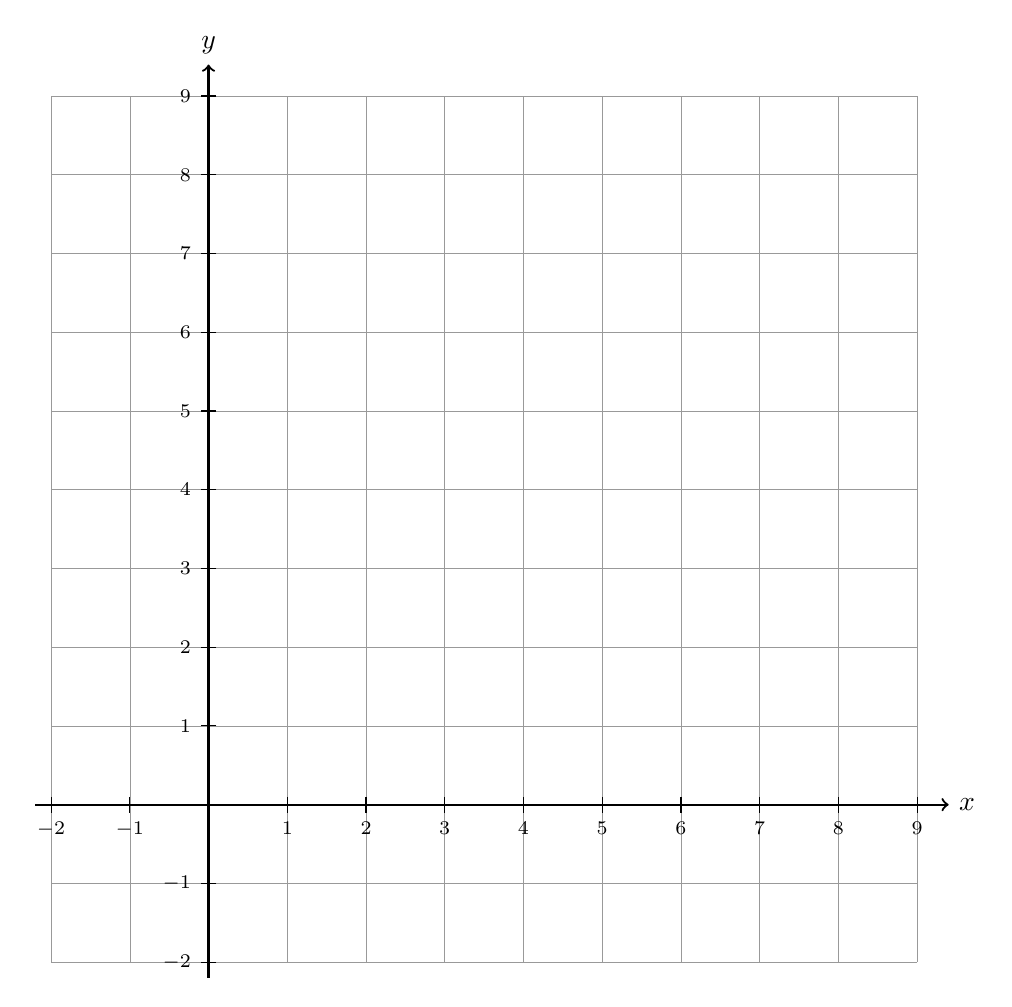
\begin{tikzpicture}[scale=1]
  \draw[very thin, gray!80] (-2,-2) grid (9,9);
  \draw[->, thick] (-2.2,0) -- (9.4,0) node[right] {$x$};
  \draw[->, thick] (0,-2.2) -- (0,9.4) node[above] {$y$};
  \foreach \x in {-2,-1,1,2,3,4,5,6,7,8,9}
    \draw (\x,0.1) -- (\x,-0.1) node[below, font=\scriptsize] {$\x$};
  \foreach \y in {-2,-1,1,2,3,4,5,6,7,8,9}
    \draw (0.1,\y) -- (-0.1,\y) node[left, font=\scriptsize] {$\y$};
\end{tikzpicture}
\end{center}

\newpage

%--- Problem 4: Use logs to solve for the input to an exponential ---
\item[4.] \textbf{Solve for the exponent}

When $x$ is in the exponent, take the logarithm of both sides. Give
exact answers.

\textbf{(a)} Solve $2^x = 20$.

\vspace{4cm}

\textbf{(b)} Solve $5^{\,x-1} = 12$.

\vspace{4cm}

\textbf{(c)} A bacteria culture is modelled by $P(t) = 50 \cdot 2^{\,t}$,
where $t$ is the time in hours. Find the exact value of $t$ at which
$P = 1500$.

\vspace{4cm}

\textbf{(d)} Solve $5^{\,2x} = 3^{\,x+1}$.

\vspace{4cm}

\end{enumerate}
\end{document}
